\newpage
\section{Three-dimensional flat plate}
\label{chapter-3Dflatplate}
%
This test case is a 3D extension of a previous 2D test case, featuring Mach 4.5 air flow across a two-dimensional flat plate. The original 2D flat plate test case is an example included in the Eilmer3 CFD suite to demonstrate the $k$-$\omega$ turbulence model. 

The example includes experimentally validated flow data extracted at $x=0.368$\,m from Mabey's 7402 series test case (documented by Fernholz and Finley~\cite{Fernholz1977}), skin friction coefficient data by Van Driest~\cite{vanDriest1956}, as well as post-processed and graphed results for the original 2D simulation. This provides sufficient information for comparison and validation of the three-dimensional extended case. 
%------------------------------------------------------------------
\subsection{Details of flow problem}
%\label{}
Figure~\ref{f:tc1:scheme} indicates the basic schematic for the flat plate flow. For the original 2D simulation, the fluid domain was specified as a single $x$-$y$ slice with a length ($x$) of $0.4$\,m. 
%
\begin{figure}[htbp]
 \begin{center}
  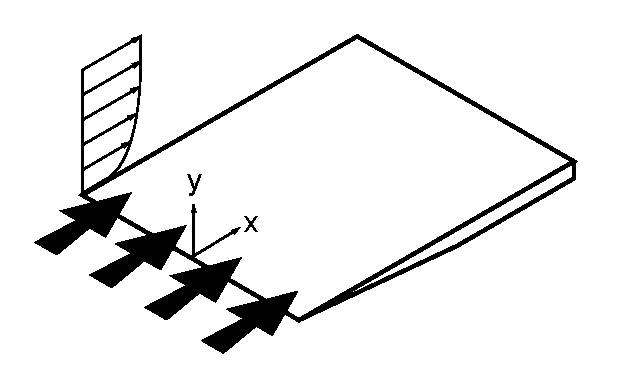
\includegraphics[width=9cm]{./chap6-3Dflatplate/figs/schematic2.pdf}
  \caption{Basic Schematic for Flat Plate Simulations.}
  \label{f:tc1:scheme}
 \end{center}
\end{figure}
%
A segment of fluid around the plate was selected using a new co-ordinate system, as indicated in Figure~\ref{f:tc1:fluid}, and inverted, resulting in the flat plate edge shifting to the top of the fluid domain. The wedged shape was used to allow viscous effects at the plate's leading edge to be properly realised, by providing sufficient space for any shocks or boundary layers to form without errors due to the domain size. 
%
\begin{figure}[htbp]
 \begin{center}
  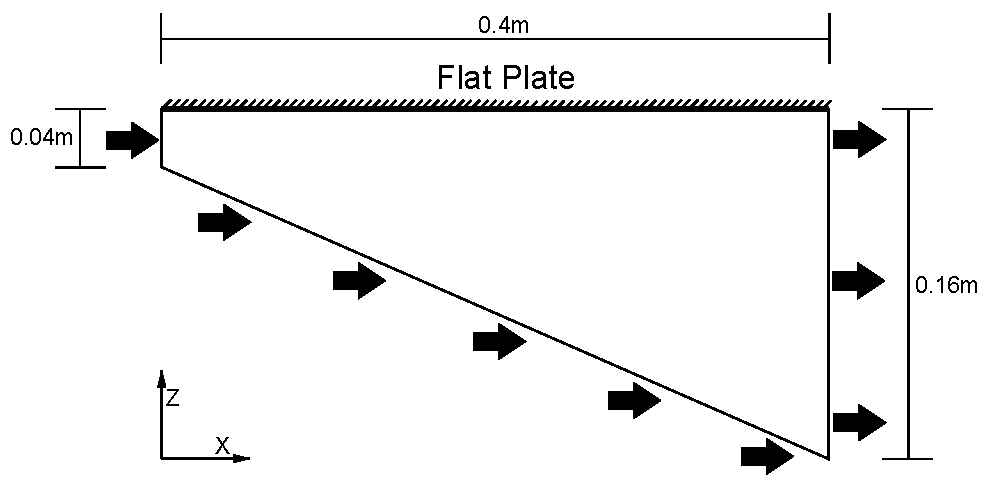
\includegraphics[width=12cm]{./chap6-3Dflatplate/figs/fluidvolume.pdf}
  \caption{Fluid Domain for 2D Flat Plate Simulation (not to scale).}
  \label{f:tc1:fluid}
 \end{center}
\end{figure}
%

For the 3D case, the selected domain was extended in the $Y$ direction by $0.01$\,m to capture flow along a strip of the plate. All other dimensions were kept identical in order to allow proper replication of the 2D results. The flow properties from the 2D flat plate, including pressure, velocity, temperature and density, were utilised by the 3D flat plate case as initial and inflow conditions (Table~\ref{t:tc1:initial}) in an attempt to ensure the results from both cases were identical.
%
\begin{table}[htbp]
  \caption{3D Flat Plate Initial \& Inflow (Freestream) Conditions.}
  \label{t:tc1:initial}
  \begin{center}
  \begin{tabular}{cccl}
  \hline\hline
     Parameter  & Value & Units \\
  \hline
    $P_\infty$  & $3.160$ & kPa  \\
    $U_\infty$  & $712.9$ & m/s  \\
    $T_\infty$  & $62.16$ & K  \\
    $\rho_\infty$  & $0.177$ & kg/m$^3$  \\
  \hline\hline
  \end{tabular}
  \end{center}
\end{table}

%
The turbulence variables $k$ and $\omega$ were initialised using a turbulence intensity of $1\%$ and turbulent-to-laminar viscosity ratio of $1$, as in the 2D flat plate case. Table~\ref{t:tc1:turb} indicates the estimated turbulence quantities used by the 3D flat plate as initial conditions.
%
\begin{table}[htbp]
  \caption{3D Flat Plate Initial (Freestream) Turbulence Properties.}
  \label{t:tc1:turb}
  \begin{center}
  \begin{tabular}{cccl}
  \hline\hline
     Parameter  & Value & Units \\
  \hline
    Turbulence Kinetic Energy ($k$)  & $76.23$ & m$^2$/s$^2$  \\
    Specific Dissipation Rate ($\omega$)  & $32.65\times10^5$ & /s  \\
  \hline\hline
  \end{tabular}
  \end{center}
\end{table}
%

\subsection{Details of computational approach}
%\label{}
The fluid domain geometry from the 2D test case of $0.4$\,m$\times0.16$\,m (with the leading edge side raised $0.12$\,m) was altered to include the 3D extension of $0.01$\,m. The co-ordinates and representative control volume were utilised in the Eilmer3 simulation, as indicated in Figure~\ref{f:tc1:geometry}.
%
\begin{figure}[htbp]
 \begin{center}
  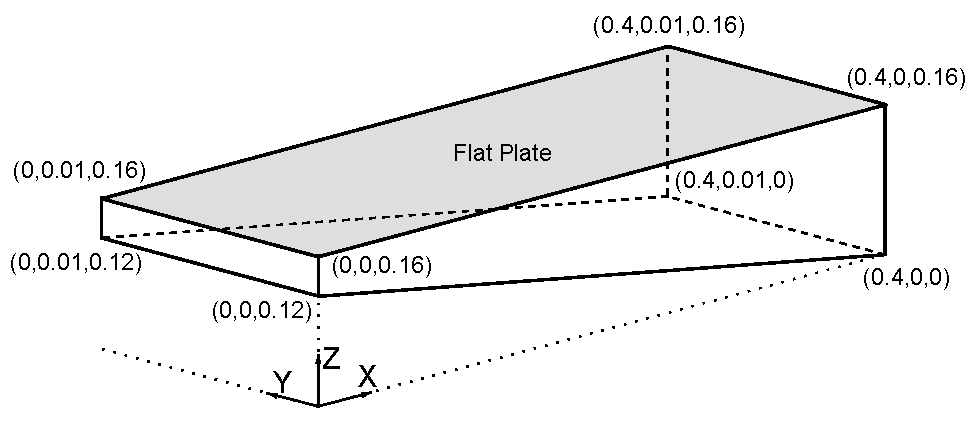
\includegraphics[width=12cm]{./chap6-3Dflatplate/figs/3Dcoordinates.pdf}
  \caption{3D Flat Plate Mesh Geometry (not to scale).}
  \label{f:tc1:geometry}
 \end{center}
\end{figure}
%
Following the 2D Flat Plate example, the geometry was divided into a $128\times96$ grid extended into 3D by 10 cells, resulting in an overall grid resolution of $128\times96\times10$ (122880) cells (Figure~\ref{f:tc1:mesh}). 
The top face of the fluid domain was represented as an adiabatic wall, the west and bottom faces as supersonic inflow, and the east face as supersonic outflow as indicated in Figures~\ref{f:tc1:fluid} and~\ref{f:tc1:geometry}. Both the north and south boundaries were set as slip walls to ensure no interference with the fluid flow, and allow the 2D results to be representative of a 'slice' of the 3D solution due to uniformity along the domain width.
%
\begin{figure}[htbp]
 \begin{center}
  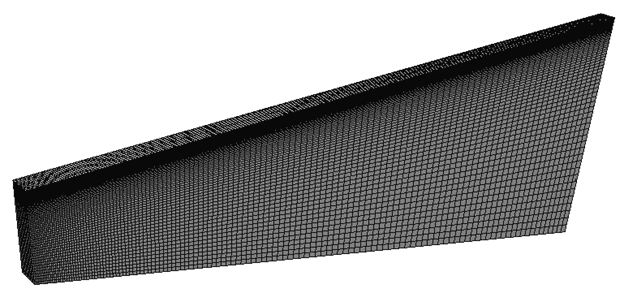
\includegraphics[width=12cm]{./chap6-3Dflatplate/figs/tc1meshbw.png}
  \caption{3D Flat Plate Simulation Mesh.}
  \label{f:tc1:mesh}
 \end{center}
\end{figure}
%
As per the 2D test case, clustering towards the leading edge and flat plate was utilised in order to ensure the $y^+<1$ criteria was met, to accurately simulate turbulence (Figure~\ref{f:tc1:mesh}). Clustering along the $Y$ direction in the 3D case was not necessary, as the north and south surfaces do not experience viscous effects.

In order to minimise simulation time, the fluid domain was split into sixteen individual blocks, to be solved separately using sixteen simultaneous threads of the Eilmer3 solver. The main block was divided into four sub-blocks along the $X$ axis and two sub-blocks along the $Y$ and $Z$ axes ($4\times2\times2$). Due to the clustering in the $X$ and $Z$ directions towards the leading edge and surface of the flat plate, the sub-blocks were differently sized in the $X$ and $Z$ directions, but equally spaced in the $Y$ direction.

\subsection{Grid convergence}
%\label{}
A grid convergence study was completed using the full resolution and a $20\%$ reduced version ($100\times8\times76$). An investigation into skin friction coefficient ($C_f$) between the two versions indicated a maximum divergence of $5\%$ during the leading edge peaks, and an average difference of $<1\%$ (Figures~\ref{f:tc1:res} and~\ref{f:tc1:comp}). Mach number, pressure, temperature and velocity comparisons did not indicate convergence (Figure~\ref{f:tc1:convergence}), as the difference in boundary layer thickness shows the effect grid resolution has on turbulent transition. The full resolution was concluded to be sufficient, as the goal of Test Case 1 was to replicate another simulation's results, not refine them. 
%
\begin{figure}[h]
 \begin{center}
  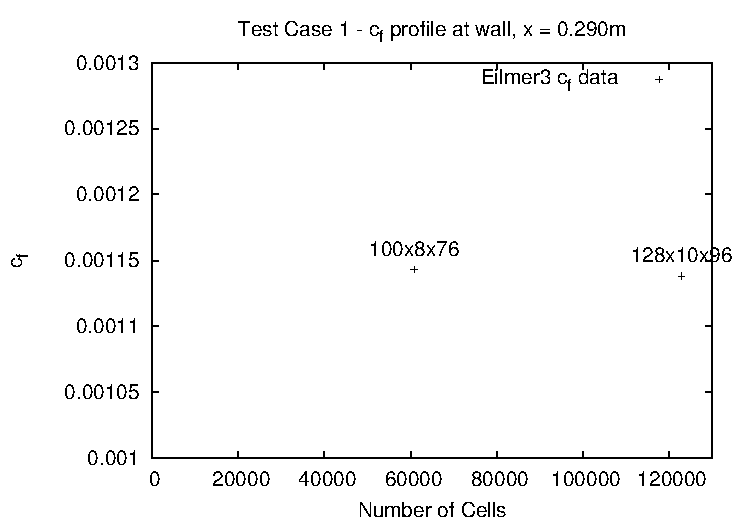
\includegraphics[width=9.2cm]{./chap6-3Dflatplate/figs/tc1-cf-resolution.pdf}
  \caption{3D Flat Plate Grid Convergence - $C_f$ at $x=0.290$\,m.}
  \label{f:tc1:res}
  \vspace{1cm}
  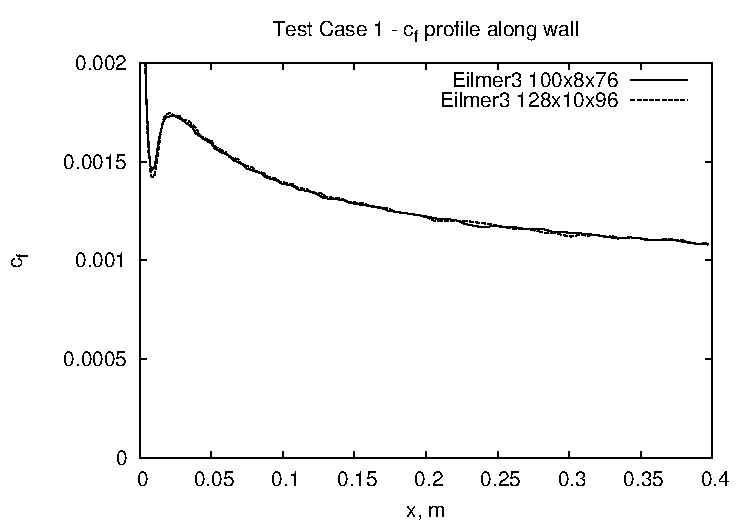
\includegraphics[width=9.2cm]{./chap6-3Dflatplate/figs/gridconverge/tc1-cf-comparison.pdf}
  \caption{3D Flat Plate Grid Convergence - Surface $C_f$.}
  \label{f:tc1:comp}
 \end{center}
\end{figure}
%
\begin{figure}[p]
 \centering
 \subfigure[Mach Number.]{
   \label{}
%   \fbox{Contents of first subfigure}
   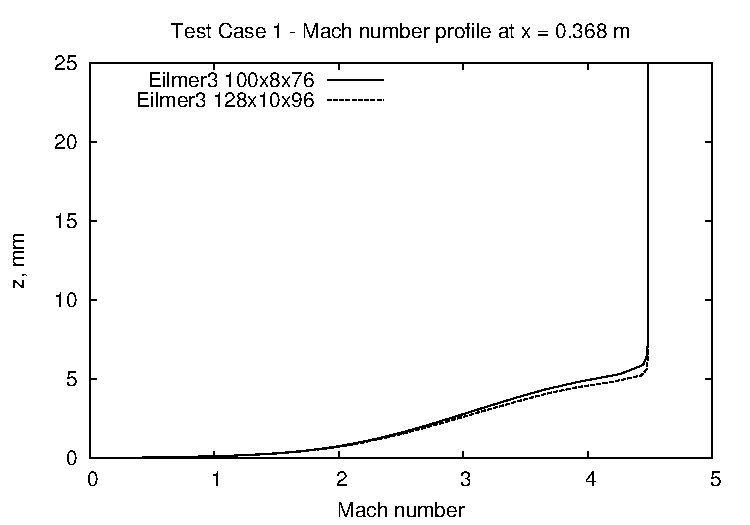
\includegraphics[width=7.5cm]{./chap6-3Dflatplate/figs/gridconverge/tc1-mach-comparison.pdf}
 }
 \subfigure[Pitot Pressure.]{
   \label{}
%   \fbox{Contents of second subfigure}
 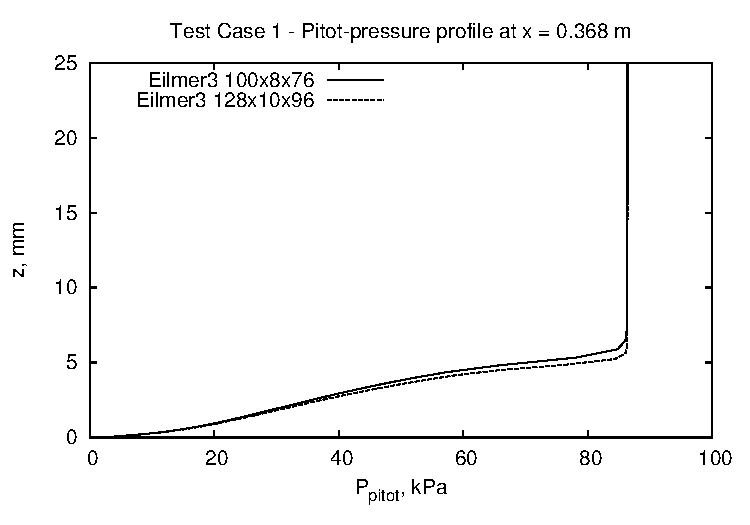
\includegraphics[width=7.5cm]{./chap6-3Dflatplate/figs/gridconverge/tc1-pitot-comparison.pdf}
 }
 \subfigure[Temperature.]{
   \label{}
%   \fbox{Contents of first subfigure}
   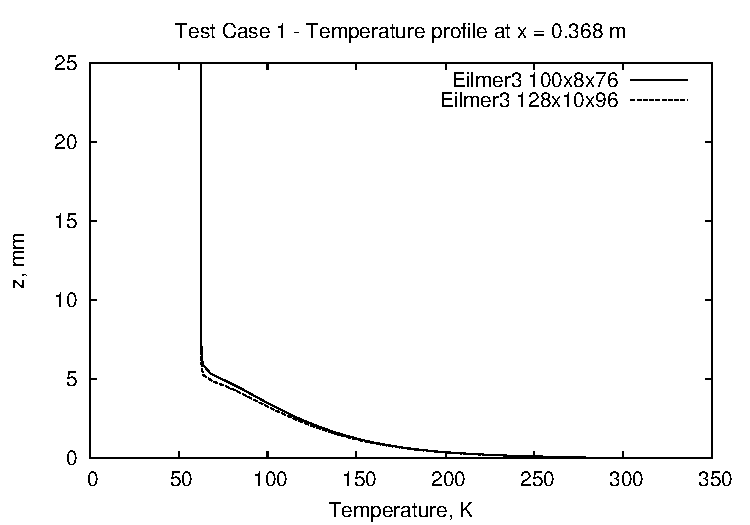
\includegraphics[width=7.5cm]{./chap6-3Dflatplate/figs/gridconverge/tc1-temp-comparison.pdf}
 }
 \subfigure[Velocity.]{
   \label{}
%   \fbox{Contents of second subfigure}
 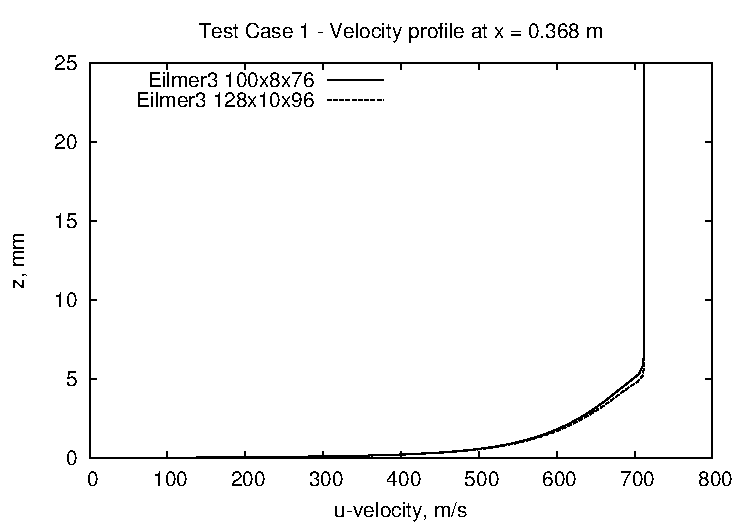
\includegraphics[width=7.5cm]{./chap6-3Dflatplate/figs/gridconverge/tc1-u-comparison.pdf}
 }
 \caption{3D Flat Plate Grid Convergence - Flow Properties.}
 \label{f:tc1:convergence}
\end{figure}

\clearpage
\subsection{Results \& discussion}
%\label{}
The flow field was tested for $1.68$ milliseconds (approximately three flow lengths), to ensure steady-state conditions were reached. This was achieved via simulation on `Barrine' for $177.78$ hours ($2844.53$ CPU-hours). Paraview was used to view the Mach number (Figure~\ref{f:tc1:mach}) and pressure (Figure~\ref{f:tc1:pressure}) data at steady-state.
%
\begin{figure}[htbp]
 \begin{center}
  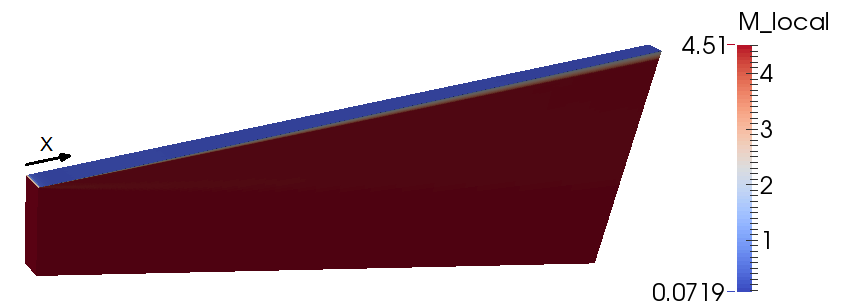
\includegraphics[width=16cm]{./chap6-3Dflatplate/figs/testcase1mach2.png}
  \caption{3D Flat Plate Mach Data.}
  \label{f:tc1:mach}
 \end{center}
\end{figure}
%

As indicated in Figure~\ref{f:tc1:mach}, the top edge of the fluid domain has a very low Mach number, due to the presence of the flat plate and turbulent boundary layer. The reduction in velocity associated with the boundary layer is present, which can be observed increasing in thickness along the $X$ axis.
A weak oblique shock, caused by the high speed flow interaction with the leading edge of the flat plate, is indicated as a slight change in velocity parallel to the bottom  boundary.
%
\begin{figure}[htbp]
 \begin{center}
  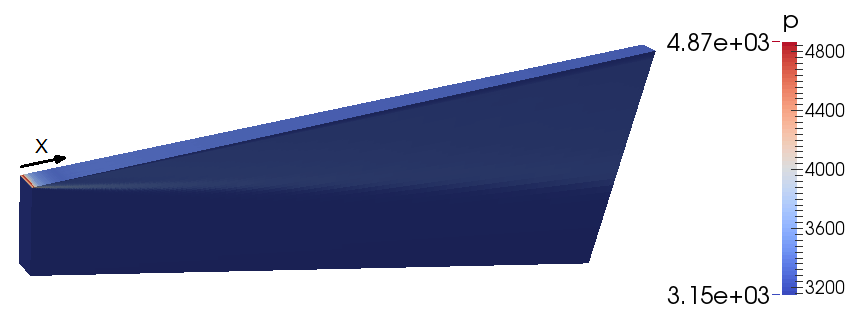
\includegraphics[width=16cm]{./chap6-3Dflatplate/figs/testcase1pressure2.png}
  \caption{3D Flat Plate Pressure Data.}
  \label{f:tc1:pressure}
 \end{center}
\end{figure}
%
Figure~\ref{f:tc1:pressure} illustrates the pressure difference over the flow domain. As with Mach number, the top surface illustrates a low pressure due to the presence of a turbulent boundary layer. The shock is much more prominent, as an increase in pressure can be observed immediately behind the shock.

Utilising a post-processing script and a modified viscous properties calculator, $X$-$Z$ slices were taken at each cell in the $Y$ direction and plotted together, in order to validate that the extension into 3D did not affect the results.
%
\begin{figure}[htbp]
 \begin{center}
  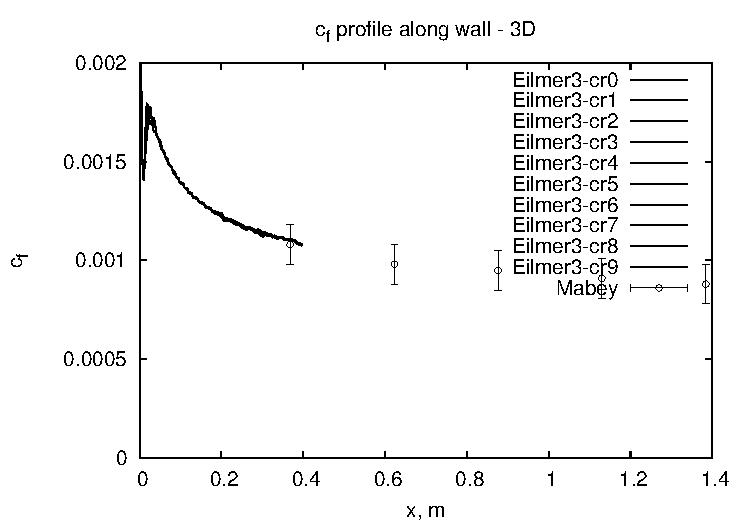
\includegraphics[width=10cm]{./chap6-3Dflatplate/figs/3Dslices/mabey-cf.pdf}
  \caption{3D Flat Plate Surface $C_f$.}
  \label{f:tc1:cf}
 \end{center}
\end{figure}
%
Skin friction coefficient ($C_f$) was extracted along the flat plate surface ($y=0.16$\,m), while temperature, Mach number, pitot pressure and velocity were extracted from a vertical slice $0.368$\,m from the leading edge, in order to allow a comparison with Mabey's experimental data. Excellent similarity was observed between the slices, as indicated by the $C_f$ data in Figure~\ref{f:tc1:cf} and other properties in Figure~\ref{f:tc1:profiles}. 

Deviation between the slices depended on the cell position, with the largest deviation in $C_f$ (of the order $10^{-4}$) occurring at the peak during boundary layer transition. Mach number, temperature, pitot pressure and velocity featured zero deviation far from the flat-plate surface, but grew as distance to the plate decreased, to the orders of $10^{-4}$, $10^{-1}$\,K, $10^{-1}$\,Pa and $10^{-2}$\,m/s at the surface respectively.
%
\begin{figure} %[htbp]%
	\centering
	\subfigure[][Mach number (M) vs. Height (mm).]{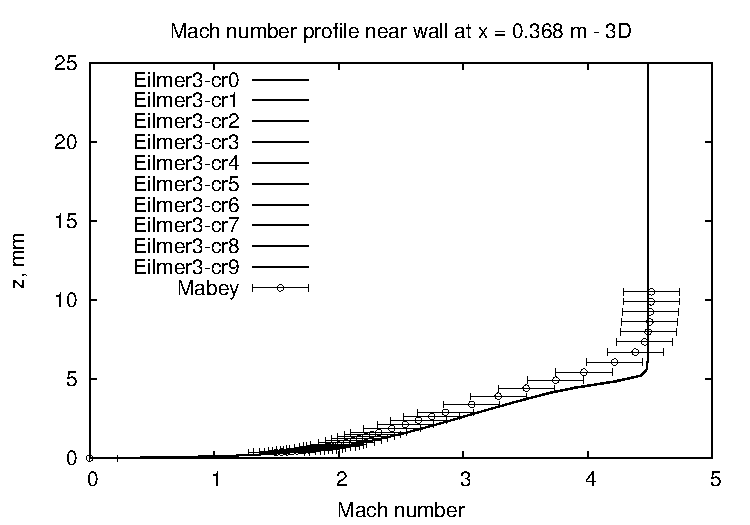
\includegraphics[width=7.5cm]{./chap6-3Dflatplate/figs/3Dslices/mabey-mach.pdf}}%
	\qquad
	\subfigure[][Velocity (m/s) vs. Height (mm).]{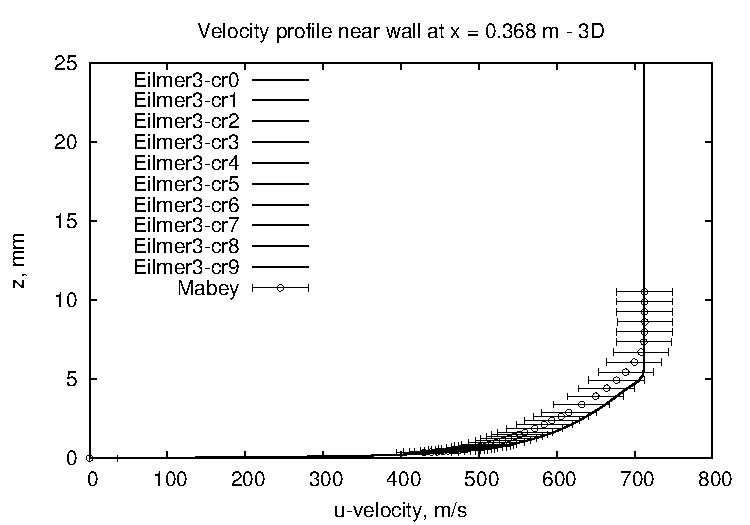
\includegraphics[width=7.5cm]{./chap6-3Dflatplate/figs/3Dslices/mabey-u.pdf}}
	
	\subfigure[][Pitot Pressure (kPa) vs. Height (mm).]{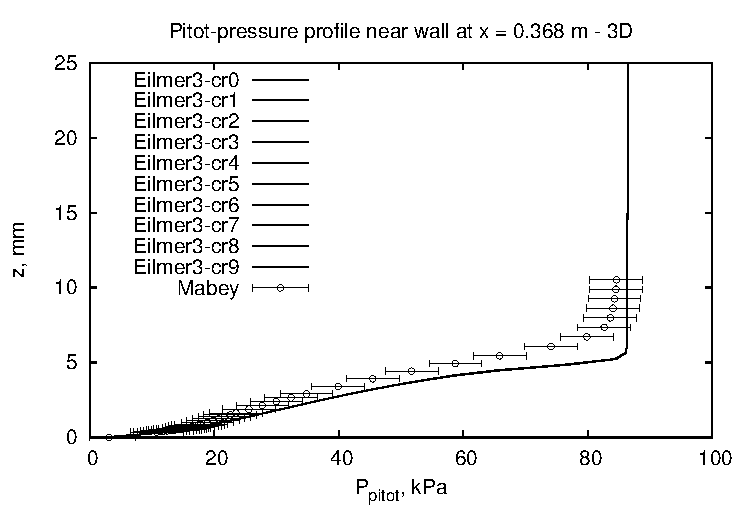
\includegraphics[width=7.5cm]{./chap6-3Dflatplate/figs/3Dslices/mabey-pitot.pdf}}%
	\qquad
	\subfigure[][Temperature (K) vs Height (mm).]{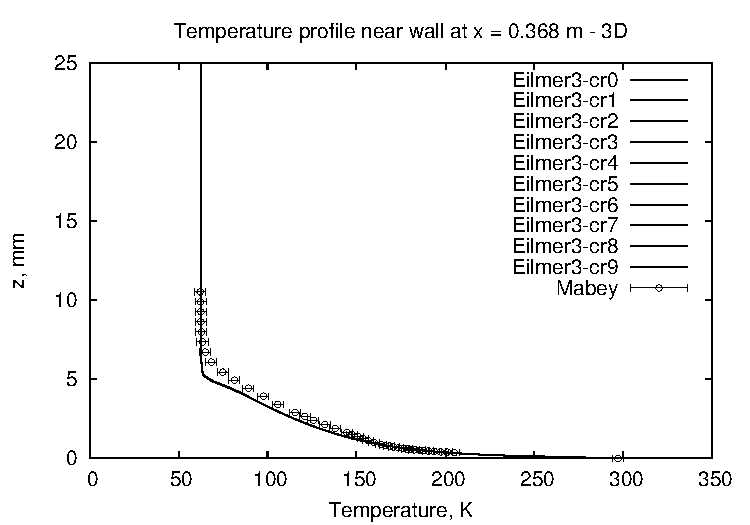
\includegraphics[width=7.5cm]{./chap6-3Dflatplate/figs/3Dslices/mabey-temperature.pdf}}
	\caption{3D Flat Plate Boundary Layer Profiles at $x=0.368$\,m.}%
	\label{f:tc1:profiles}%
\end{figure}
%
Once the internal 3D validation was completed, the comparison between the 2D and 3D
flow schemes was undertaken. This comparison was made by graphing the original 2D test case data with a single slice from the 3D flat plate. As shown in Figure~\ref{f:tc1:2Dv3Dprofiles}, the 2D and 3D data for Mach number, temperature, pitot pressure and velocity correlate well at $x=0.368$\,m, while Figure~\ref{f:tc1:2Dv3Dcf} indicates a noticeable difference in skin friction coefficient along the flat-plate between the simulations.
Far-field values for Mach number, temperature, pitot pressure and velocity feature zero deviation between the simulations , but grew to the order of $10^{-3}$, $10^{-1}$\,K, $10^1$\,Pa and $10^{-1}$\,m/s respectively at the flat plate surface. 

By extending the flat plate into three dimensions, velocity had transformed from a 2D vector to a 3D vector. Data analysis indicated that $Y$ velocity components arose in the 3D simulation which were not present in 2D, as well as a reduction in the $X$ and $Z$ velocity components.  The $Y$ velocities in the far-field are of the order of $10^{-9}$\,m/s, however are observed to peak at $10^{-3}$\,m/s close to the flat plate surface and fluctuate between positive and negative values as the distance from the leading edge increases. Due to skin friction coefficient's dependence on parallel ($X$ direction) velocity and temperature, these large deviations observed at the surface are expected to be the cause of the $10^{-4}$ deviation in $C_f$ seen in Figure~\ref{f:tc1:2Dv3Dcf}.
%
\begin{figure}[htbp]
 \begin{center}
  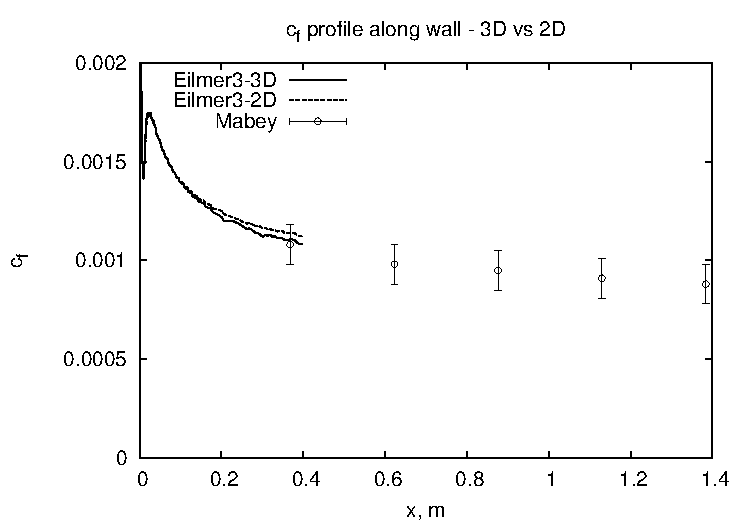
\includegraphics[width=10cm]{./chap6-3Dflatplate/figs/2Dto3D/mabey-cf1.pdf}
  \caption{3D vs 2D Flat Plate Surface $C_f$.}
  \label{f:tc1:2Dv3Dcf}
 \end{center}
\end{figure}
%

While the 2D flat plate results weren't replicated perfectly, extending the case into 3D altered the turbulent flow effects and identified a limitation of the three-dimensional turbulence simulation. It was expected that there would be no $Y$ velocity components due to flow symmetry, as the 2D flat plate extension into 3D represented an ideal `slice'. The observed difference in skin friction coefficient indicated the development of $Y$ velocity components within the turbulent boundary layer, identifying a potential bug in the solver. 
%
\begin{figure} [htbp]
	\centering
	\subfigure[][Mach number (M) vs. Height (mm).]{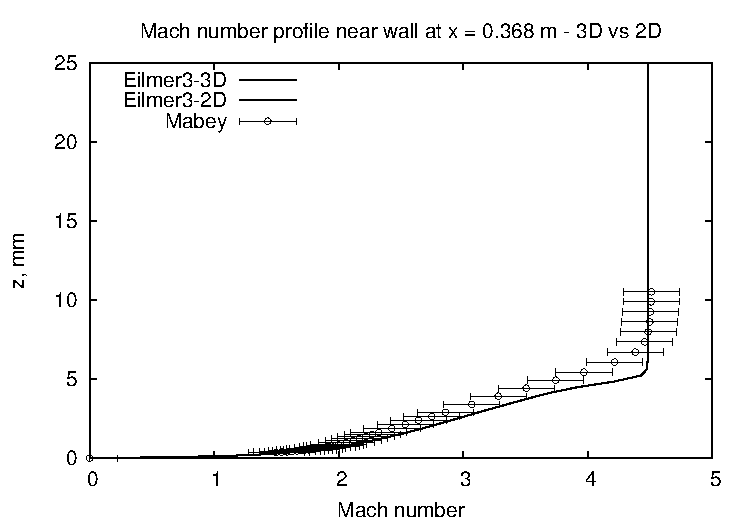
\includegraphics[width=7.5cm]{./chap6-3Dflatplate/figs/2Dto3D/mabey-mach.pdf}}%
	\qquad
	\subfigure[][Velocity (m/s) vs. Height (mm).]{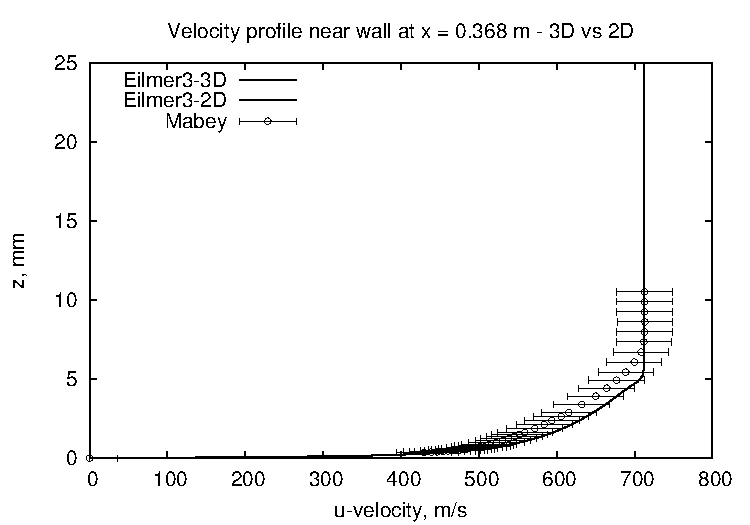
\includegraphics[width=7.5cm]{./chap6-3Dflatplate/figs/2Dto3D/mabey-u.pdf}}
	
	\subfigure[][Pitot Pressure (kPa) vs. Height (mm).]{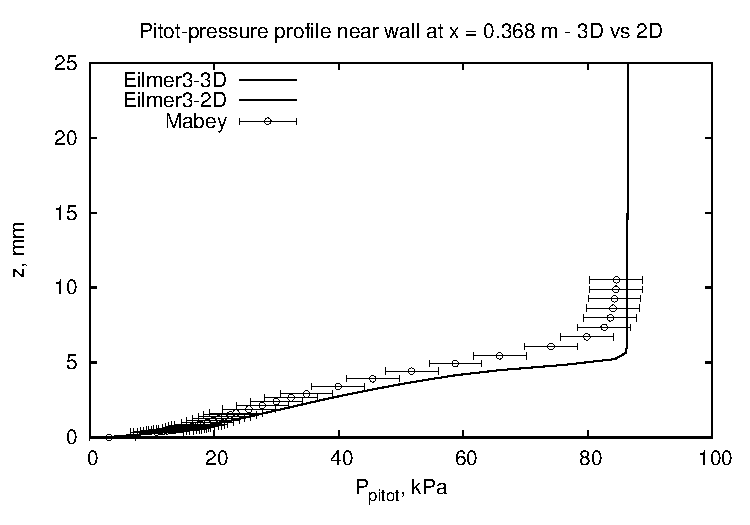
\includegraphics[width=7.5cm]{./chap6-3Dflatplate/figs/2Dto3D/mabey-pitot.pdf}}%
	\qquad
	\subfigure[][Temperature (K) vs Height (mm).]{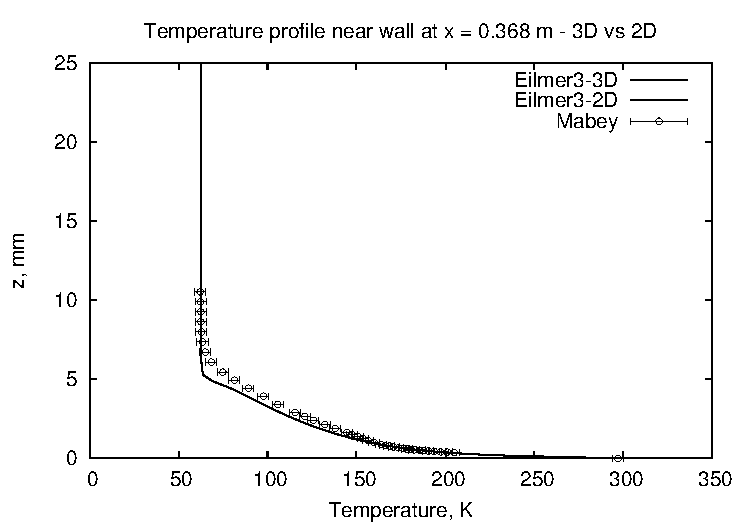
\includegraphics[width=7.5cm]{./chap6-3Dflatplate/figs/2Dto3D/mabey-temperature.pdf}}
	\caption{3D vs 2D Flat Plate Boundary Layer Profiles at $x=0.368$\,m.}%
	\label{f:tc1:2Dv3Dprofiles}%
\end{figure}